\documentclass{acm_proc_article-sp}
\usepackage{graphicx}
\usepackage{listings}
\usepackage{hyperref}
\usepackage{algorithmicx}
\usepackage{algpseudocode}
\usepackage{algorithm}
\usepackage{url}
\usepackage{listings}
\usepackage{color}

% definitions
\def \tool {InputFinder}  
\def \numbinaries {24}

\begin{document}

\title{InputFinder: Reverse Engineering Closed Binaries via Side Channels}
%\numberofauthors{2}
%\author{
%\alignauthor
%Bogdan Copos\\
%	\affaddr{University of California, Davis}\\
%	\email{bcopos@ucdavis.edu}
%\alignauthor
%Praveen Murthy\\
%	\affaddr{Fujitsu Laboratories of America}\\
%	\email{praveen.murthy@us.fujitsu.com}
%}
\maketitle

\begin{abstract}
The effectiveness of many dynamic program analysis techniques depends heavily on the completeness of the test suite applied during the analysis process.
Test suites are often composed by developers and aim at testing all of the functionality of a software system.
However, test suites may not be complete, if they exist at all.
To date, only two methods exist for automatically generating test input for closed binaries: fuzzing and symbolic execution.
Despite previous successes of these methods in identifying bugs, both techniques have limitations.
In this paper, we propose a new method for autonomously generating valid input and identifying protocols for closed x86 binaries.
To assess its effectiveness, we have developed \tool{} and tested it against binaries from the DARPA Cyber Grand Challenge example set.
Our evaluations show that our method is not only effective in finding input and determining whether a protocol is expected but can also find unexpected control flow paths.
\end{abstract}

\section{Introduction}
%introduction
Vulnerability testing is an expensive and labor intensive process.
For many years, researchers have explored both static and dynamic methods for analyzing programs \cite{smartfuzzer}.
While static analysis can be more thorough, dynamic testing is often preferred due to its time efficiency.
However, dynamic testing heavily depends on the availability of appropriate inputs or test suites.

%motivation
Without complete test suites, the program cannot be properly tested and some bugs may be omitted during testing.
While valid input can be learned from software documentation or source code, when such information is not available or complete, other methods must be used.
Automated dynamic analysis techniques such as fuzzing and symbolic execution attempt to generate input for a given program.
Currently these are the only two options available and both approaches present limitations.
Fuzzing done randomly with no inference attempted of the program's behavior cannot be effective as the input space is usually too large.
Symbolic execution has traditionally been used with manual intervention to identify potential symbolic variables to begin exploration with, a luxury we do not have when analyzing closed binaries autonomously, in addition to scalability issues and limitations of decision procedures that are used to solve the constraints.

In this paper, we introduce a new method, called InputFinder, for generating valid user-input for closed binaries. 
This new method could be useful in autonomous vulnerability scanning systems, or for reverse engineering unknown binaries.
Our method is composed of two main components.
The first component exploits side channels to build valid input for closed binaries.
Specifically, as the program is given various inputs, \tool{} records the number of instructions \textbf{retired} during the program's execution for each input and uses a statistical measure to infer the program's expected input.
The number of instructions retired differs from the number of instructions executed by a processing unit.
Because of the out-of-order CPU pipeline, a CPU may execute more instructions than necessary (e.g. as a result of wrong branch prediction).
The instructions retired represent the subset of instructions executed which leave the \textit{Retirement Unit} once execution has been deemed correct (i.e. the instructions which actually impact the program).
The same side channel is used by \tool{} to also find the expected input size and to categorize the expected input based on type.
The second component uses the discovered input to build a protocol state machine associated with the tested program.
This enables the generation of a more thorough test suite.

The main contributions of this paper are as follows:
\begin{itemize}
	\item We introduce a new approach to automatically generate input valid strings for unknown, closed-source binaries by leveraging hardware instruction counters. Our method relies on observing changes in the number of instructions retired by programs during their input validation process to learn valid input strings.
	\item We describe how our method can be used not only to find valid input strings, but also to determine the expect input size and classify input based on type (e.g. alphabetic, alphanumeric, numeric, etc.).
	\item We develop a method for generating protocol state machines using the valid input previously found.
	\item We implement the techniques presented as a proof of concept tool and evaluate it using binaries published by DARPA as part of the 2014 Cyber Grand Challenge competition \cite{darpacgc}. Additionally, we compare our approach to the manual process used by a security specialist to crack a binary as part of a job interview \cite{interviewbinary}.
\end{itemize}

The paper is organized as follows.
Section \ref{prevwork} discusses related works and highlights differences between the related works and the work presented here.
Section \ref{background} covers background information relating to concepts utilized in this work.
The details of our approach are explained in Section \ref{methodology}. First, the method for finding valid input is described. Then we introduce our method for building protocol state machines using the discovered input.
Section \ref{results} describes the evaluation of the work presented and the results.
In Section \ref{futurework}, we share future plans for our work and explain cases which the proposed method does not handle.


\section{Previous Work} \label{prevwork}
Dynamic analysis is extensively studied in academia and is used widely in the industry by security specialists.
Two of the main approaches to vulnerability testing are fuzzing and symbolic execution.

Fuzzers are a popular choice amongst software testers.
They are easy to use, easy to implement, and can produce surprising results \cite{millerfuzz, millerfuzzrevisited}.
There are two classes of fuzzers: black box fuzzers and white box fuzzers.
In black box fuzzing, the program is watched as it is tested with randomly generated input.
If the program crashes, the input(s) are recorded and reported.
No prior program specifications or knowledge of the input format is available in such cases.
Since black box fuzzing is completely random, its effectiveness is limited, especially with respect to coverage.

Symbolic execution is another method used for generating valid input.
When a program analyzer symbolically executes a program, it does not use concrete values.
Instead, the input is represented as a mathematical formula composed of symbols and equations resulting from the constraints (related to the input) gathered during the program's execution.
Specifically, the tester first marks the input as symbolic.
This can also be done automatically via taint analysis.
The program is then executed by an interpreter that assumes symbolic values for those symbolic input locations.
As the program executes, whenever operations are performed on those symbolic variables, a formula in terms of those symbols keeps track of the mathematical operations performed on the symbolic variables.
The formula can also have constraints on those symbols based on outcomes of conditional branches encountered during the executions.
At the end of execution, or during certain portions of the execution, the formula is examined by a constraint solver to determine whether it is satisfiable (meaning that a solution exists to make the formula true), and if it does, concrete values for all symbolic variables in the formula are computed.
Those concrete values will then constitute a set of test cases that can execute the program along the set of paths (because of branches) encountered in the formula.
Symbolic execution has been proven effective by previous works \cite{symbolicexecution, exesymex}.
One of the most important works in this area is described in \cite{exesymex} which introduces EXE, a dynamic analysis tool capable of generating inputs that crash programs by running the programs with symbolic input.

White box fuzzing leverages the symbolic execution traces of a given binary to produce more inputs.
One of the many previous works is \cite{godefroid2008automated} which introduces SAGE, an automated white box fuzzer.
White box fuzzing differs from black box fuzzing in that it uses the concrete inputs to gather constraints and then systematically negates constraint clauses to generate additional inputs that cover more branches in the program.
White box fuzzing can attain better code coverage but can be slow.
Symbolic execution (and consequently white box fuzzing) is crippled by innate limitations of constraint solvers.
While symbolic execution engines perform well with linear constraints, non-linear constraints greatly impact efficiency.
One of the works utilizing white box fuzzing is \cite{molnar2009dynamic} which introduces SmartFuzz, a dynamic test generation tool.
SmartFuzz uses symbolic execution to learn about the program's input and passes that information to a fuzzer for test case generation.

The main difference between our work and SmartFuzz is that our work does not use symbolic execution to gain insight into the format of the input.
Similar to SmartFuzz, the output of our work can be used by a fuzzer to generate test cases.
Unlike the EXE symbolic execution engine, the SAGE tool, and SmartFuzz, the approach presented in our work is not hindered by constraint solvers.
Additionally, compared to EXE, our method does not require any instrumentation or source code.
\tool{} does not execute the program with symbolic input but rather it bootstraps itself by building up a set of valid inputs (from an initially empty set) by gathering information about the execution of a program.

Another related work is presented in \cite{smartfuzzer}, where the authors use a combination of static and dynamic analysis to build a smart fuzzer.
Their work uses static analysis to collect preliminary information such as an approximation of the inter procedural control flow graph.
Having gathered static information, their dynamic analysis engine executes the program while monitoring dependencies between the input and the dynamic control flow path experienced by the program.
Their work also takes advantage of a constraint solver that, given a path of the program, generates input which forces the program to follow the chosen path.
Our work \tool{} differs from their approach in several ways.
One difference is that our work uses neither static analysis nor constraint solvers.
Instead our input finding method relies only on information extracted from the execution of the un-instrumented program. 

There have also been numerous works studying and applying dynamic similarity.
In \cite{blanketexec}, the authors propose blanket execution, a novel dynamic equivalence testing technique.
Blanket execution is designed to collect information about the execution of functions, including side effects, which is then used for similarity testing.
Another important work is \cite{differential} which introduces \textit{differential slicing} for the purpose of identifying flow and value differences across multiple executions of the same program for security applications.
Both our approach and the previous approaches mentioned above use a dynamic approach to gather information about the program.
However, our approach aims at finding differences in executions of a given program in order to make inferences about the underlying protocol expected by the program.
This allows us to discover the orders of inputs which experience unique control flow paths.

Another area of research relevant to this paper is protocol reverse engineering.
An important result in this area is \cite{prospex} which introduces a technique for extracting protocol specifications from packet captures and automatically generating input which can be used by a stateful fuzzer.
There are two notable differences between Prospex and our work.
While the end result is similar, \tool{} assumes no prior knowledge about the tested program and hence it does not utilize packet captures for protocol specification extraction.
Instead, \tool{} infers the protocol through dynamic analysis by automatically finding input and using that to generate a protocol state machine.
Caballero et. al introduce Polyglot \cite{polyglot}, a tool that uses dynamic binary analysis to observe how programs process the received application data and uses that information to infer the protocol's message format.
Their work is similar because of the use of dynamic binary analysis and the use of information from program traces to make inferences about the protocol format.
However, our work does not try to determine the protocol message format but rather the high level protocol.
Additionally, unlike Polyglot, our work does not use test cases or previously known input.
To date, we do not know of any protocol reverse engineering techniques which work without any prior knowledge about the program's input.

\section{Background} \label{background}

\subsection{Side Channels} \label{bg_sidechannels}
Side channels are streams of information that can be retrieved from the hardware of a device running a given program.
This information can be used to gather knowledge regarding the program's internal components.
Side channels have been widely explored by security researchers in order to discover weaknesses in programs \cite{weinbergside, schindler2002combined, genkin2014rsa, genkinstealing}.
In cryptography, side channel attacks exploit such information channels to defeat crypto systems \cite{zhou2005side, black2002black, okeya2006side}.
Recently, side channel attacks, such as OpenSSL's CREAM cache timing attack have made headlines \cite{creamssl}.
Similar to CREAM and other side channel attacks, the technique discussed in this paper exploits such information channels to generate valid input for binaries.
\subsection{Hardware counter registers} \label{bg_hardwarereg}
Most modern microprocessors are equipped with a set of special-purpose registers used to count hardware events.
Each register, or counter, can be programmed to measure specific events such as cache misses, floating point operations, and even instructions retired.
Such hardware performance counters are often used by software developers to analyze their programs and improve the running time and efficiency.
However, in this paper we show how such performance counters can also be exploited as side channels.
Utilities, such as Linux/Unix \textit{perf}, take advantage of such hardware counters in order to provide developers with useful information about a program's performance.
The \textit{perf} utility allows developers to specify the desired hardware event they wish to measure.
Once events have been selected, \textit{perf} interacts with the appropriate kernel modules to program the hardware counters accordingly.
In this work, we use \textit{perf} to count the number of \textbf{user-land} instructions retired as a program is tested with various input.
\textbf{User-land} instructions are instructions of a program which run outside the operating system's kernel.
While other options are available for counting instructions retired, we choose \textit{perf} for its efficiency and minimal overhead.
The number of \textit{total} instructions retired varies significantly for a binary from execution to execution \cite{weaver2008can}.
This phenomenon reflects fluctuations in instructions retired by the kernel depending on the state of the machine due to cache-misses and other factors.
Since we rely on this count, such variations are problematic.
However, experimentally, the number of \textit{user-land} instructions only varies, on average, by one instruction, giving us a reliable counter.
\subsection{Execution/Dynamic Matching} \label{bg_dynamicsim}
In many application areas, including clone detection and software debugging, there is a need for comparing executions of a program (or multiple versions of a program).
One of the proposed approaches aimed at tackling this issue is dynamic matching.
Dynamic matching works by first collecting execution traces of different executions.
Such traces can be collected through a number of ways.
One option includes the use of a tool such as \textit{Pin} \cite{pintool}.
\textit{Pin} is a framework for building customized binary analysis tools and can be used to design a tool which creates a transcript of the instructions retired by a program.
Once the traces are collected, they are analyze and mappings between instructions of different executions are produced.
These mappings can be used to understand the relationship between two executions (or two versions of a program).
In this work, we rely on the concept of dynamic matching and the \textit{Pin} framework to develop a protocol state machine generator for closed binaries.

\section{Methodology} \label{methodology}

\tool{} is composed of two main modules.
The first module is responsible for discovering input and properties of the expected input, including input size and the type of the input.
The input generated by the first module is then used by the second module to generate a protocol state machine.
The protocol state machine can be used by third party tools such as stateful fuzzers for even better code coverage.
\subsection{Finding Valid Input}
The majority of software programs accept input, perform transformations on the input, and output results.
However, most programs do not accept completely random input.
Input usually passes through an input validation filter.
Such filters are snippets of code responsible for distinguishing between valid or good input (i.e. input the program was constructed to understand and accept) and bad input (i.e. input which is not useful or does not follow the desired format).
Although validation mechanisms can be very sophisticated, they are often a combination of string comparisons and conditional statements.
Code snippets of input validation from our tested binaries can be found in Appendix A.
Our method exploits changes in the number of user-land instructions retired during multiple executions with varying inputs to make inferences about the program's validation mechanism.
These changes reflect different execution paths of the program as a response to both valid and invalid input.
Assuming most input is invalid, our method observes differences in the number of instructions retired to detect input which passes the validation mechanism.

\begin{figure*}[t]
\centering
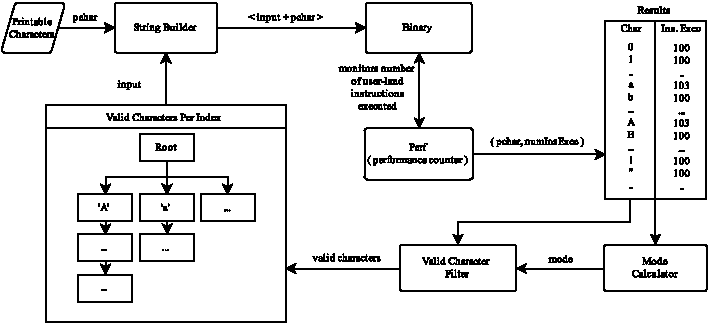
\includegraphics[width=\textwidth]{architecture.pdf}
\caption{This figure depicts the architecture of the finding input process. There are three main parts: the input string builder, the performance counter (i.e. \textit{perf} utility), and the valid character filter}
\label{fig:architecture}
\end{figure*}

Figure \ref{fig:architecture} shows the overall architecture of the finding input component of \tool{}.

\begin{algorithm}
\caption{Pseudocode implementing the input finding process}
\label{findinputcode}
\begin{algorithmic}[1]
\State $s \leftarrow ``"$ \Comment{starting with an empty string}
\Procedure{FindInput}{$s$}
\For{i=0, \Call{size}{$printableChars$}} %\Comment{for all printable character}
\State char = printableChars[$i$]
\State insRetired = \Call{ExecBin}{$s+char$} \label{execute}%\Comment{execute binary with input $s+char$}
\State insPerInput[$char$] = insRetired %\Comment{record number of instructions retired}
\EndFor
\State mode = \Call{CalcMode}{$insPerInput$} \label{mode}%\Comment{calculate mode across all executions}
\For{i=0, \Call{size}{$printableChars$}} \label{filterbegin}%\Comment{for all printable character}
\State char = printableChars[$i$]
\State count = insPerInput[$char$]
\If{mode-epsilon < count < mode+epsilon}
\State ignore
\Else
\State validCharList += char
\EndIf
\EndFor \label{filterend}
\If{no valid characters found}
\State end of string reached
\State return
\Else
\For{i=0, \Call{size}{$validCharList$}} \label{fork}
\State validChar = validCharList[$i$]
\State \Call{FindInput}{$s+validChar$}
\EndFor
\EndIf
\EndProcedure
\end{algorithmic}
\end{algorithm}

% \algref{findinputcode}{line}
The steps of the process for finding valid input are described in algorithm \ref{findinputcode} and outlined below. Starting with an empty string, \textit{s}:
\begin{enumerate}
\item \tool{} executes the program once for every printable character and records the number of user-land instructions retired by the program with the given input. The input is a string concatenation of the string \textit{s} and the current printable character. The Unix \textit{perf} utility is used for monitoring the number of instructions retired. Note that \tool{} does not record the total number of instructions but rather user-land instructions. The reason for this, as explained in Section \ref{bg_hardwarereg}, is in contrast to user-land instructions, that the total number of instructions retired can vary greatly from execution to execution for various reasons (e.g. branch prediction, cache). The Expect tool is used for automating the program interaction. This step is shown in line \ref{execute} of algorithm \ref{findinputcode}.
\item Once all executions have been completed (one for each character), the mode number of instructions retired is computed across all executions. The mode is defined as the value that appears most often in the set of recordings. This is done in line \ref{mode} of algorithm \ref{findinputcode}.
\item Next is the filtering stage which is responsible for identifying characters likely to be part of a valid input string at the current index. Under the assumption that most characters are not valid for the current index, \tool{} gathers all characters with the number of instructions retired outside the range of the mode +/- an epsilon value, as shown in lines \ref{filterbegin}-\ref{filterend} of algorithm \ref{findinputcode}. These characters represent valid characters for the current index of the input string. The epsilon value accounts for small variations in the hardware counters. While the initial reaction is to expect a valid character to result in more instructions retired than a non-valid character, this is not always the case. As discussed earlier, the input validation mechanism can be complex and can vary in behavior. The validation mechanism may verify input against all accepted input strings before denying the provided input. Such a scenario results in more instructions retired for invalid input than valid input.
\item For each valid character \textit{c}, \tool{} forks, with every child process repeating steps 1-4, starting with $ c + s $ as the initial input string, where $+$ signifies concatenation (starting at line \ref{fork} of algorithm \ref{findinputcode}). If no valid characters are found, the end of a valid input string has been reached and the string is recorded. If the current index is 0 and no valid characters have been found, the given binary has no predefined input commands.
\end{enumerate}

\begin{figure*}[t]
\centering
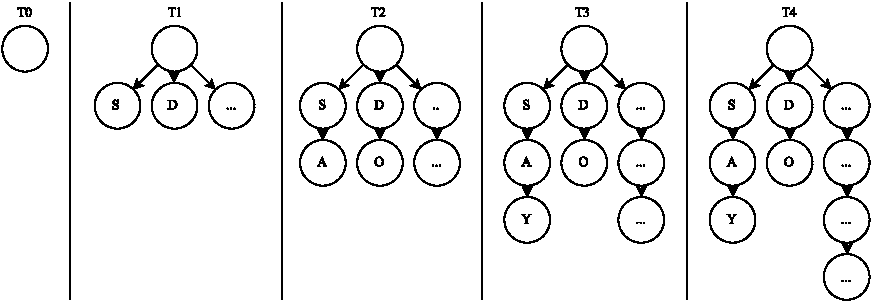
\includegraphics[width=\textwidth]{string_builder.pdf}
\caption{This diagram visualizes the input strings being constructed throughout five consecutive time stages of the execution of 
\tool{}. Multiple outgoing arrows represent a process forking. This occurs when multiple valid characters are detected for a given index of the input string and, as a result, the finding input process forks to concurrently handle all of the discovered characters.}
\label{fig:string_builder}
\end{figure*}

Figure~\ref{fig:string_builder} depicts the results of the above process over the span of five consecutive time stages.
As seen in the figure, at time \textit{T0}, \tool{} begins with an empty string.
At time \textit{T1}, \tool{} finds valid characters for index 0 of the input string and is forked into \textit{n} child processes where \textit{n} is the number of valid characters found.
This continues until all child processes are done.

\subsubsection{Finding Desired Input Size}
The same side channels can be used to detect the expected size of the program's input or even the size of the program's input buffer.
Specifically, there is a change in the behavior of the program with respect to the number of instructions retired when the size of the input is larger than expected.
Most programs are designed to read a predefined number of bytes from the source of input and store the read bytes in a buffer.
A popular way of doing that is by using the \textit{fgets()} or \textit{scanf()} functions of the GNU C stdio library.
As the input size grows, the number of instructions retired also increases linearly.
This happens because additional instructions are needed to read more characters from the input source.
However, when the input string is larger than the expected size, the number of instructions retired no longer increases as a function of the input size.
This behavior can be observed and exploited to find the expected input size, which may often also be the size of the input buffer.
Our method observes such differences in the number of user-land instructions retired as the program is given increasingly larger input.

To start, \tool{} finds the set of all invalid characters for index 0 of all input strings and picks one at random.
The character selected is used to build invalid input strings of various sizes.
It is crucial to use invalid input to avoid noisy fluctuations in the number of instructions retired due to valid input processing.
Initially, the program is executed twice: once with an input string of two invalid characters and once with an input string of three invalid characters.
The number of user-land instructions retired during these two executions are recorded.
These two values may be equal or different, depending on the program's logic.
The two values may be equal if, for example, the program uses the system call \textit{read()} directly to read data from the input file descriptor.
Since we are measuring the number of user-land instructions retired (not also instructions retired by the kernel), the instructions retired by the \textit{read()} function are not included in our counter so there will be no linear increase in the number of instructions retired as the input size is increased.
If the two values are equal, the program is executed with increasingly large input until a change in the number of executions is recorded due to the program logic.
If the values differ (as discussed earlier), the difference in the number of instructions retired is recorded and the program is executed, increasing the size of the input, until a change is detected.
Instead of increasing the input size linearly, the input size is increased exponentially until a change is detected.
Once the change is detected, the input size is decreased to find the exact size at which the change happens.
It is also possible that the number of instructions retired oscillates between two (or more values).
One example is a palindrome finder.
The same underlying concept can be applied to such cases.

Determining the exact size is useful when performing symbolic execution on a buffer where one cannot make the size of the buffer symbolic (since frameworks such as \textit{Fuzzball} do not allow for that).
In such cases, being able to determine the buffer size is necessary and useful to instruct the symbolic execution engine the exact size of the buffer that should be made symbolic.
We detected 5 crash inputs in the tested binaries because of our finding input size approach.

\subsubsection{Categorizing Input}
Our method is also capable of classifying the input discovered.
Generated input strings are classified in three categories: alphabetic, numeric, alphanumeric.
Similarly, the classification algorithm detects special characters.
Once enough input strings have been identified, \tool{} uses the categorization data to generalize about the type of input the program accepts.
This is done by iterating through the characters of the input strings discovered and determining which category they fall into.
Such information is valuable especially in cases where the inputs discovered are all numeric or contain (one or more) special characters.
Having learned such information about the program, the testing platform (e.g. fuzzer) can be adjusted to proceed accordingly.

\subsection{Generating Protocol State Machine}
Thus far, we have described how \tool{} discovers valid input for a given binary autonomously.
However, some binaries have an implicit protocol.
Consider, for example, a database management program.
Without first selecting a database and perhaps even a table, some commands such as \textit{INSERT} or \textit{SELECT} are useless and have no effect on any data.
We develop the second component of \tool{} to address this issue.
Specifically, this component identifies expected orderings (or permutations) of the discovered input strings, and constructs a protocol state machine.

\begin{algorithm}
\caption{Pseudocode implementing the protocol state machine generator}
\label{psmcode}
\begin{algorithmic}[1]
\Procedure{main}{$inputs$}
\For{i = 1, \Call{size}{$inputs$}}
\State length = i
\State permutations = \Call{GetPermutation}{$length$}
\State results = $\emptyset$
\For{j = 0, \Call{size}{$permutations$}}
\State permutation = permutations[$j$]
\State \Call{Exec}{$permutation, 0, results$}
\EndFor
\State \Call{Compare}{$results, inputs$}
\EndFor
\EndProcedure

\Procedure{Exec}{$cmds, i, results$}
\If{ i == \Call{size}{$cmds$}}
\State results += cmds
\State return
\EndIf

\State initCmds = cmds[0:i]
\State cmd = cmds[i]
\State args = \Call{FindArgs}{$initCmds, cmd, i$}
%\Comment{find arguments for cmd, given initial commands initCmds}

\For{j=0, \Call{size}{$args$}}
\State cmds[$j$] = cmds[$j$] + arg
\State \Call{Exec}{$cmds, i+1, results$}
\EndFor
\EndProcedure

\Procedure{Compare}{$results, inputs$}
\For{i=0, \Call{size}{$results$}}
\State cmds = results[$i$]
\State lastCmd = cmds[\Call{size}{$cmds$}-1]
\State trace = \Call{ExecBinWithPin}{$cmds$}
\State traceForLastCmd = \Call{SplitTrace}{$trace, cmds$}
\State allTraces[$lastCmd$][$cmds$] = traceForLastCmd
\EndFor
\For{i=0, \Call{size}{$inputs$}}
\State cmd = inputs[$i$]
\For{j=0, \Call{size}{$allTraces[cmd]$}}
\State cmdTraces = allTraces[$cmd$][$j$]
\State clusters = \Call{Compare}{$cmdTraces$}
\State goodPermutation = \Call{Filter}{$clusters$}
\EndFor
\EndFor
\EndProcedure
\end{algorithmic}
\end{algorithm}

\begin{figure}[h!]
\caption{Architecture of the protocol state machine generator}
\centering
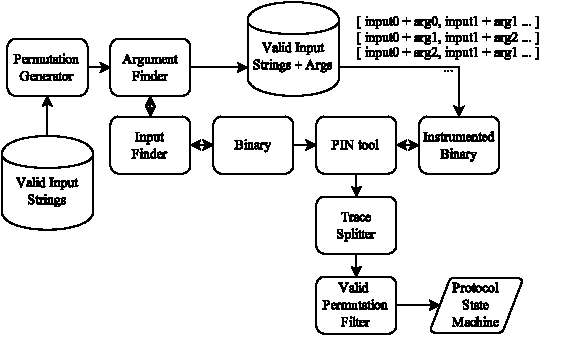
\includegraphics[width=0.53\textwidth]{psmarch.pdf}
\label{fig:psm_arch}
\end{figure}

The architecture of this component is depicted in Figure \ref{fig:psm_arch}.
The process is described below and shown as pseudocode in algorithm \ref{psmcode}.
First, all possible permutations of all sizes from 2 to the number of input strings discovered are computed (e.g. given input strings $a,b,c,d$, the permutations generated include [a,b] , [a,c] , [a,d] , [b,a] , [b,c] , [b,d] ... [a,b,c] , [a,b,d], [a,c,b] ... [a,b,c,d] , ...  etc.).
Every permutation is passed through the dynamic analysis engine.
The dynamic analysis execution engine first splits the permutation into individual input strings.
Maintaining the original order of the inputs within the permutation, each string is tested for the presence of expected arguments.
For example, if the input string is \textit{SET} and the program accepts input of the format \textit{SET data}, the analysis tries to determine that \textit{data} is a valid argument by applying the input finding method with \textit{SET} as the command and identifying additional characters after the $<SPACE>$ character.
The arguments found are saved for later use.
Once every input string of a given permutation has been tested for arguments, the inputs are passed through the instrumented version of the program binary for the collection of the execution trace.
The binary is instrumented with a \textit{Pin} tool, developed by us, which logs the starting address of every basic block executed, as a function of time.
A basic block is a set of instructions with a single entry and a single exit point.
Once all permutations of a given size have been executed, the dynamic similarity test begins.
This test splits each execution trace into parts, each part being associated with an input string.
The splitting process is done by first executing the program without any input, examining the trace, and extracting a short sequence of basic blocks from the end of the trace.
The sequence of basic blocks extracted is used as the delimiter during the splitting process and it represents the basic blocks executed by the program right before reading and processing the user input.
We refer to the execution trace of the input string \textit{SET} as $\alpha(SET)$.
For all permutations of the same size with the same last input string, the traces $\alpha(lastCmd)$ are clustered.
Given a permutation $p$ of size $s$ let $\alpha(p_s)$ represent the execution trace of the command at index $s$ of the permutation (i.e. last command of the permutation).
Take for example two different permutations $p1$ and $p2$.
Both permutations are of the same length, $i$.
Both permutations are composed of the same input strings and have the same last input string (e.g. [a,b,c,d] vs. [b,a,c,d]).
Assume permutation $p1$ represents the correct (or expected) order of the input strings.
It is natural to assume that the input string $p_i$ (i.e. last input string in the permutation) experiences a different execution trace (or control flow path) as a result of permutation $p1$ than permutation $p2$.
This information is used to determine, for every input string discovered, if there exists a permutation which affects its control flow path.
If such a permutation is discovered, it is added to the protocol state machine.

\begin{figure}[h!]
\caption{Example of protocol state machine for one of the DARPA Cyber Grand Challenge example binaries.}
\centering
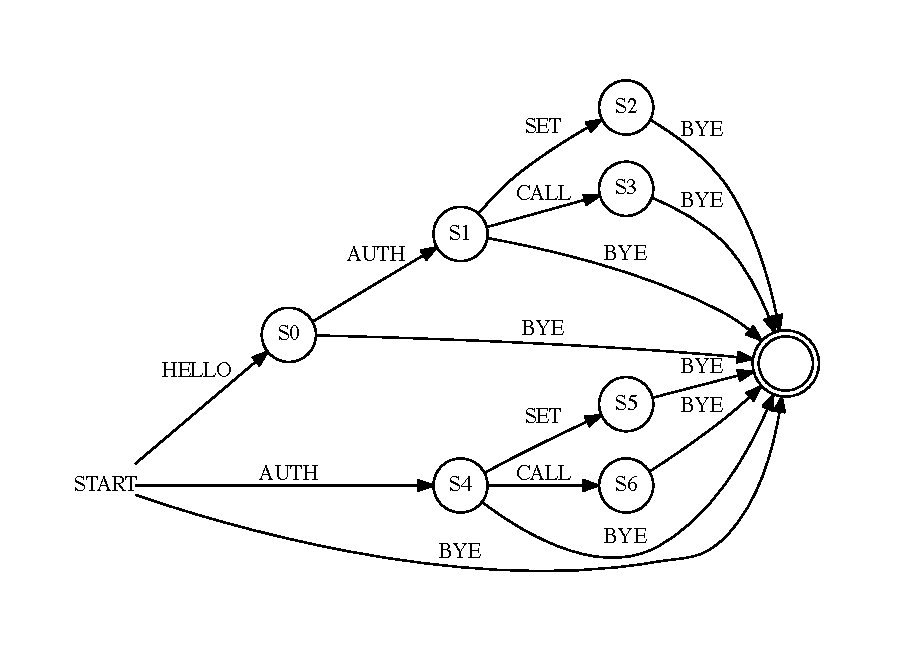
\includegraphics[width=0.53\textwidth]{protocoldiagram.pdf}
\label{fig:psm_example}
\end{figure}

An example of a protocol state machine can be seen in Figure \ref{fig:psm_example}.
Since there is no information about the states and their meaning, the states are represented by circles with generic names (e.g. $S0$).
The arrows represent input strings that enable the transition between states.

\section{Evaluation and Results} \label{results}
\subsection{Finding Input, Input Size and Classifying Input}
In order to determine its effectiveness, \tool{} was tested on \numbinaries{} x86 binaries from the DARPA Cyber Grand Challenge Example set \cite{darpacgc}.
The Cyber Grand Challenge (CGC) binaries are 32 bit x86 binaries in the CGC format.
The only difference between the CGC format and the well known ELF format is in the header of the binaries and in the fact that dynamic linking is not supported.
Additionally, they are designed to only be executed in the Cyber Grand Challenge platform and utilize different system calls than the UNIX system calls.
The Cyber Grand Challenge organizers also provide the source code of the binaries which, with some effort, can be modified to use UNIX system calls and be built as ELF x86 binaries.

The results are summarized in Table \ref{binaryresults}.
Analyzing the source code showed that out of the \numbinaries{} binaries, 21 had predefined valid input strings.
\tool{} found input strings for 13 of the 21 binaries and categorized the input correctly for 100\% of the 13 binaries.
The running time varied between a few minutes and an hour, depending on the number and length of the valid input strings discovered.
Our method was able to determine the input length for 19 of the 24 binaries.
Note that the our approach was able to find the expected input length even if it was not able to find valid input.
Additionally, our method was able to determine crash inputs for 5 of the binaries.
In all cases, the crash input caused a buffer overflow and caused the binary to exit unexpectedly.

\begin{table*}
\centering
\begin{tabular}{|c|c|c|c|c|c|} \hline
\textbf{Binary} & \textbf{Input} & \textbf{Number of Inputs} & \textbf{Input Size} & \textbf{Crash Input} & \textbf{Protocol State Machine}\\ \hline
06459301 & yes (8 min) & 8 out of 8 & yes & no & -\\ \hline
06b71301 & no & - & yes & no & -\\ \hline
07a9a901 & - & - & yes & yes & - \\ \hline
0b32aa01 & yes (2 min) & 1 out of 1 & yes & yes & - \\ \hline
11dc8e01 & no & - & yes & no & - \\ \hline
1877a601 & yes (11 min) & 6 out of 6 & yes & no & - \\ \hline
250d1101 & yes (20 min) & 5 out of 5 & yes & no & yes \\ \hline
2eca0101 & yes (42 min) & 7 out of 7 & no & no & - \\ \hline
37e97201 & yes (38 min) & 6 out of 6 & yes & no & - \\ \hline
3dcf1a01 & yes (6 min) & 6 out of 6 & yes & yes & - \\ \hline
48b9cf01 & yes (50 min) & 9 out of 9 & yes & no & - \\ \hline
65884701 & no & - & no & no & - \\ \hline
701b7301 & - & - & yes & no & - \\ \hline
7262d006 & yes (5 min) & 4 out of 5 & yes & no & - \\ \hline
7fa39f01 & no & - & yes & yes & - \\ \hline
b8993403 & yes (12 min) & 1 out of 1 & yes & no & - \\ \hline
badd9e01 & no & - & yes & no & - \\ \hline
caea9c01 & no & - & yes & no &  -\\ \hline
cc366801 & yes (60 min) & 10 out of 10& no & no & - \\ \hline
d476cd01 & no & - & yes & no & - \\ \hline
df9df201 & no & - & yes & no & - \\ \hline
e7cd3901 & - & - & no & yes & - \\ \hline
f14eb101 & yes (53 min) & 11 out of 11 & no & no & yes \\ \hline
f658d801 & yes (2 min) & 1 out of 4 & yes & no & - \\
\hline\end{tabular}
\caption{The table describes the results of our evaluation. The \textit{Input} column describes whether our approach was able to discover valid input strings. As previously mentioned, some binaries did not have any predefined input strings (hence such binaries are marked by the \textit{-} in this column). The \textit{Number of Inputs} column describes how many input strings our method discovered out of the total number of input strings defined by the binary.}
\label{binaryresults}
\end{table*}

Additionally, our input finding method was tested on a binary used for technical interviews.
The binary was designed as a reverse engineering challenge for interviewees.
To pass the challenge, the interviewee has to crack the secret passcode to the program.
A blog post describes the manual process used by one interviewee to crack the password \cite{interviewbinary}.
The manual process is tedious and it includes methods such as disassembling the binary, stepping through the instructions using a debugger, and reverse engineering the logic of the program.
As described in the blog post, the cracking of the binary can take several hours and requires advanced skills and years of background knowledge.
\tool{} was able to crack the binary in a matter of minutes autonomously.

\subsection{Protocol State Machine Generation}
The evaluation of the protocol state machine generator was also done using the DARPA Cyber Grand Challenge binaries.
However, out of the total of \numbinaries{} binaries, only 2 had a clear implicit protocol.
Specifically, these 2 binaries requested authentication before allowing full functionality.
Our method was able to generate a correct protocol state machine for both of these binaries.
The protocol state machine generated was manually verified against the source code of the binaries.

\subsection{Case Study}
To further prove the usefulness of the method presented in this paper, we use one of the Cyber Grand Challenge binaries (i.e. 250d1101) as a case study and for comparison with a black-box fuzzer and a symbolic execution engine.
The binary implements a simple protocol that lets the user call functions applying root64 and parcour schemes.
The binary is built such that after sending the \textit{HELLO} command, it will generate an authentication token which is echoed to the user and must be used for the \textit{AUTH} command.
Without proper authentication, the \textit{SET} and \textit{CALL} commands have no effect.
Before generating the protocol state machine, \tool{} analyzed the binary and discovered the input strings $HELLO, AUTH, SET, CALL$, and $BYE$ in approximately 20 minutes.
These inputs are the only inputs implemented by the binary's protocol.
The protocol state machine generator not only determined that authentication is necessary but also discovered that a user can properly authenticate themselves with a value of 0 or any special character if they omit the \textit{HELLO} command (Figure \ref{fig:psm_example}).
This shows that the input finding approach in combination with the protocol state machine generator can help identify potential backdoors or unexpected control flow paths for a given program.

When comparing our method with a black box fuzzer and a symbolic execution engine, we ran each technique for 30 minutes and gathered code coverage statistics.
The black box fuzzer used is the open source \textit{zzuf} fuzzer and the symbolic execution engine used is that of the \textit{Fuzzball} \cite{zzuf, fuzzball}.
While most popular for its symbolic execution, \textit{Fuzzball} is a tool for binary analysis, built on top of the BitBlaze Vine \cite{bitblaze, bitblazesite}, which can do a number of things including extracting various traces and computing coverage statistics.
For simplicity reasons, we use the \textit{Fuzzball} tool to collect code coverage statistics.
For compatibility reasons with the \textit{Fuzzball} tool, we translated the source code of the binary to use UNIX system calls and compiled it in the ELF format.
The changes are minor and have no impact on the functionality of the program.

The results of the comparison show that \textit{zzuf} covered a total of 8936 basic blocks and was unable to discover any valid input strings.
At the same time, the \textit{Fuzzball} symbolic execution engine executed a total of 9922 and 10003 basic blocks (explained below) and was able to discover the valid input strings.
The method presented in this paper executed 10055 basic blocks and not only discovered value input strings but also identified that a user can authenticate themselves with the command \textit{AUTH 0}.

It should be noted that while the fuzzer and our method worked autonomously, the \textit{Fuzzball} symbolic executioner required some reverse engineering of the program to help setup.
One of the important parameters needed for symbolic execution was the address (and size) of the memory desired to be treated as symbolic.
The different values of the basic blocks executed by \textit{Fuzzball} are due to multiple executions of the engine with varying parameters.
Overall, the results prove that the method presented in this paper is efficient with respect to both time and code coverage.

\section{Future Work and Limitations} \label{futurework}
While the method presented in this paper has many advantages, it also has a few limitations.
For certain programs that allow any input, such as an echo server, our method is not any more efficient than a black box fuzzer.
Additionally, our method cannot handle cases in which input is composed of multiple inter-dependent fields, such as when the value of a field determines the length of another field and when binaries validate input fields out of order.
This is one reason why our method failed to detect input for some of the binaries tested.
Another reason of failure is binaries which accept non printable input (e.g. hex characters, binary, etc.).

One may argue that there are other ways of finding the input strings of a binary.
One option is the use of the Unix \textit{strings} utility, which finds all null terminated strings inside a binary.
One problem with this approach is that the \textit{strings} utility may return a number of other strings within the binary, strings not used for input validation.
Such strings can create a lot of noise and hinders the use of the \textit{strings} utility.
Additionally, our approach can find dynamically generated input strings which the static \textit{strings} utility is not capable of.
Another option is the use of the \textit{ltrace} tool which echoes library functions called and their arguments.
\textit{ltrace} could be used to determine calls of the \textit{strcmp()} function, which can help identify valid input strings.
However, a program can be implemented to dynamically detect if it is being traced by a utility such as \textit{ltrace}.
We argue that a complex input validation process can make the \textit{ltrace} and \textit{strings} utlitities less efficient than our method.
For example, one of the binaries used in the testing of our method, used a tree structure to represent valid input strings (see Appendix A, Example 2).
Each node in the tree structure represented a valid character and its depth in the tree represented its index in the input string.
Such an input checking method greatly impacts the efficiency of alternative approaches such as the \textit{strings} and the \textit{ltrace} utilities.
The \textit{strings} utility would not be useful since the input strings are represented one character at a time.
Regardless of whether the binary is designed to detect when it is being traced, using an \textit{ltrace}-based technique would also fail since the program compares characters and does not use a library function (such as \textit{strcmp()}).
On the other hand, our approach successfully finds the valid input strings despite the complexity of the input validation mechanism.

In the future, we wish to improve our current method.
First, we would like to extend to handle binary input.
Furthermore, we would like to apply the input finding technique recursively.
It is easy to imagine programs for which the second input varies based on the value of the first input.
Also, there obviously exist programs for which some inputs have no predetermined value (such as registering a username).
It would be helpful to determine such cases, provide some input and continue the execution of the program, applying the input finding technique once again.
However, there are challenges with this, such as determining when to not apply the finding input method because the program has reached an already observed and tested state.

With respect to the protocol state machine, currently our method uses the input finding technique to determine valid arguments.
However, the protocol state machine does not currently handle situations in which there are no predefined arguments (e.g. given input \textit{CREATE} the arguments could be predefined such as \textit{dog} or random such as any number).
Ultimately, we would like to generate some random arguments that remain constant for every input string in a given permutation.
Moreover, our current approach is not capable of identifying equivalent states.
As seen in Figure \ref{fig:psm_example}, the different authentication paths (use of \textit{HELLO} vs. omission of \textit{HELLO}) lead to different states when in reality the two states (i.e. user is authenticated) are identical.
Although we have not yet explored this, state minimization approaches for finite state machines may be applicable for this problem.
Also, our method is based on the assumption that given a number of input strings, the majority of input string permutations are not valid and do not reflect the expected protocol.
There may be cases where this assumption does not hold.
A better option might be to monitor other aspects of the program, particularly the \textit{.data} and the \textit{.bss} sections and the heap during the executions and see how they react to various input string permutations.
In the future, we would like to address the above mentioned concerns with our approach for generating protocol state machines.

\section{Conclusions}
This paper introduces two novel techniques for autonomously generating valid input strings for closed x86 binaries and for generating a protocol state machine using the discovered input.
For generating valid input strings, our method exploits the number of instructions retired to infer whether a given character is valid for a given index of an input string.
This process allows us to recursively and incrementally craft valid inputs.
To further gain knowledge about the user interaction with the program, we test the program with the inputs generated and construct a protocol state machine which depicts the expected order of the input strings.

We show that our proposed methods are efficient and successful by testing them on \numbinaries{} DARPA binaries from the Cyber Grand Challenge \cite{darpacgc}. 
Unlike previous works, our methods do not have any fundamental limitations (such as constraint solvers) and are robust enough to handle program binaries of other formats.

We believe that the our techniques could be applied and used in a number of settings including the building of test suites, discovering unwanted or unexpected control flow paths, and  finding bugs (when used in combination with a fuzzer).

%\section*{Acknowledgments}
%The authors would like to thank Thuan Pham for his feedback and useful discussions.

\bibliographystyle{abbrv}
\bibliography{inputfinder}

\appendix
\section{Input Validation Code Snippets}
The following are two examples of input validation mechanisms from the DARPA Cyber Grand Challenge sample binaries.

\subsection{Example 1}

In this example, we can see that the program uses the \textit{strcmp()} function to determine if the user input is a valid command.
Because of the nature of the \textit{strcmp()} function, when a character at a given index is valid (i.e. pertains to one of the commands), the function will then move to the next character of the input string and compare that with the next character of the command.
In our work, we exploit the change in the number of instructions executed caused by this to find valid input strings.

\definecolor{codegreen}{rgb}{0,0.6,0}
\definecolor{codegray}{rgb}{0.5,0.5,0.5}
\definecolor{codepurple}{rgb}{0.58,0,0.82}
\definecolor{backcolour}{rgb}{0.95,0.95,0.92}
 
\lstdefinestyle{mystyle}{
    %backgroundcolor=\color{backcolour},   
    commentstyle=\color{codegreen},
    keywordstyle=\color{magenta},
    numberstyle=\tiny\color{codegray},
    stringstyle=\color{codepurple},
    basicstyle=\footnotesize,
    breakatwhitespace=false,         
    breaklines=true,                 
    captionpos=b,                    
    keepspaces=true,                 
    numbers=left,                    
    numbersep=5pt,                  
    showspaces=false,                
    showstringspaces=false,
    showtabs=false,                  
    tabsize=2
}
 
\lstset{style=mystyle}
 
\lstinputlisting[language=C]{inputval1.txt}

\subsection{Example 2}
This example comes from a program implementing a Federal Acquisition Regulation (FAR) section lookup service.
FAR is a set of rules governing the federal government's purchasing process.
Here the system call \textit{receive()} is used to read input directly from the specified file descriptor.
The user input is parsed in the \textit{process()} function and the valid input commands are stored in a tree like structure created in the \textit{main()} function.
Since the system call is used to read the user input, the number of user-land instructions executed will not increase as a function of the input size (as it would in the previous example).
Our method is able to successfully detect both the valid input strings and the correct expected input size.
On the other hand, alternative approaches such as the \textit{strings} utility and the \textit{ltrace} tool would fail.
The \textit{strings} utility can only detect null terminated strings, not characters.
An \textit{ltrace} based method would also fail since the program compares characters and does not use a library function for this task (such as \textit{strcmp()}).


\lstinputlisting[language=C]{inputval3.txt}


\end{document}

